\chapter{Estudo de Viabilidade}
\label{cap4:avaliacao}
\pagestyle{plain}

\section{Considerações Iniciais}
Neste tópico é apresentado um estudo de viabilidade da abordagem \textit{SMartyTesting}.

Um estudo de viabilidade é essencial para verificar se existem evidências iniciais para o desenvolvimento aprofundado de determinada teoria ou tecnologia, neste caso, da abordagem \textit{SMartyTesting}. Para isso, hipóteses foram estabelecidas com base em critérios de avaliação com relação ao uso de DS e DA para a geração de sequências de teste.

\section{Objetivo}
\label{cap4sec:objetivos_avaliacao}
Com base nas considerações iniciais, o propósito principal deste estudo é analisar se \textbf{\textit{SMartyTesting} possui condições e meios para a geração de sequências de casos de teste utilizando diagramas de sequência}. 

Baseado no modelo \textit{Goal Question Metric} (GQM) \cite{basili1992software}, este estudo visa: \textbf{Caracterizar a abordagem \textit{SMartyTesting}}, \textbf{com o propósito de} identificar a sua viabilidade \textbf{com relação à} capacidade de geração de sequências de teste a partir de diagramas de sequência do ponto de vista de pesquisadores de LPS, \textbf{no contexto de} docentes e aluno de pós-graduação em Engenharia de Software da Universidade Estadual de Maringá (UEM).


\section{Planejamento}
\label{cap4sec:planejamento_avaliacao}

\subsection{Critérios de Avaliação}
\label{cap4subsec:criterios}
Para alcançar o objetivo deste estudo, foram definidos os seguintes critérios:

\begin{itemize}
	\item \textbf{CT.1:} quantidade de sequências de teste geradas. Esse critério tem como base as sequências de teste geradas por cada abordagem, em que uma sequência de teste pode apresentar um número X de casos de teste;
	\item \textbf{CT.2:} diferenciação entre sequências geradas. Quando é feita a geração das sequências, os artefatos de entrada de cada abordagem diferem uns dos outros por causa das particularidades do modelo inicial. Sendo assim, pode-se obter caminhos de sequências diferentes uns dos outros, demonstrando que foram tomados caminhos diferentes, diferenciando-se um dos outros;
	\item \textbf{CT.3:} complexidade das sequências de teste geradas. Para verificação da complexidade de um programa de computador, \citet{mccabe1976complexity} desenvolveu uma métrica para medição chamada de complexidade ciclomática, que mede a quantidade de caminhos em execução em uma aplicação. Assim, será usada essa métrica para verificar a complexidade das sequências de teste geradas; e
	\item \textbf{CT.4:} esforço no uso da abordagem para geração de sequência de teste. Quanto à medição do esforço, por meio de observação, foi verificado o tempo gasto para a utilização da abordagem desde a entrada do artefato inicial até as sequências de teste geradas. Nesse caso, verifica-se o esforço de utilização, para isso realizou-se uma observação em relação ao tempo de utilização de cada abordagem, do inicio até a geração das sequências de teste. 
\end{itemize}


\subsection{Hipóteses do Estudo}

As seguintes hipóteses foram estabelecidas de acordo com o objetivo principal deste estudo e os critérios definidos:

\begin{itemize}
	\item \textbf{Hipótese $H_{CT.1}$:} a geração de sequências fazendo uso de Diagramas de Sequência por meio da abordagem \textit{SMartyTesting} gera mais sequências de teste do que o uso de Diagramas de Atividades utilizando SPLiT-MBt;
	
	\item \textbf{Hipótese $H_{CT.2}$:} a utilização de Diagramas de Sequência por meio da abordagem \textit{SMartyTesting} cria diferenciação entre sequências de teste, em comparação aos Diagramas de Atividades com SPLiT-MBt;
	
	\item \textbf{Hipótese $H_{CT.3}$:} a utilização de Diagramas de Sequência com a abordagem \textit{SMartyTesting} gera menor complexidade das sequências de teste geradas, em comparação com os Diagramas de Atividades com SPLiT-MBt; e

	\item \textbf{Hipótese $H_{CT.4}$:} a utilização de Diagramas de Sequência com a abordagem \textit{SMartyTesting} possui menor esforço na geração de sequências de teste, comparado com o uso de Diagramas de Atividades com SPLiT-MBt.
\end{itemize}

A \ref{fig:hipoteses} ilustra as abordagens e as hipóteses definidas.

\begin{figure}[H]
	\centering
	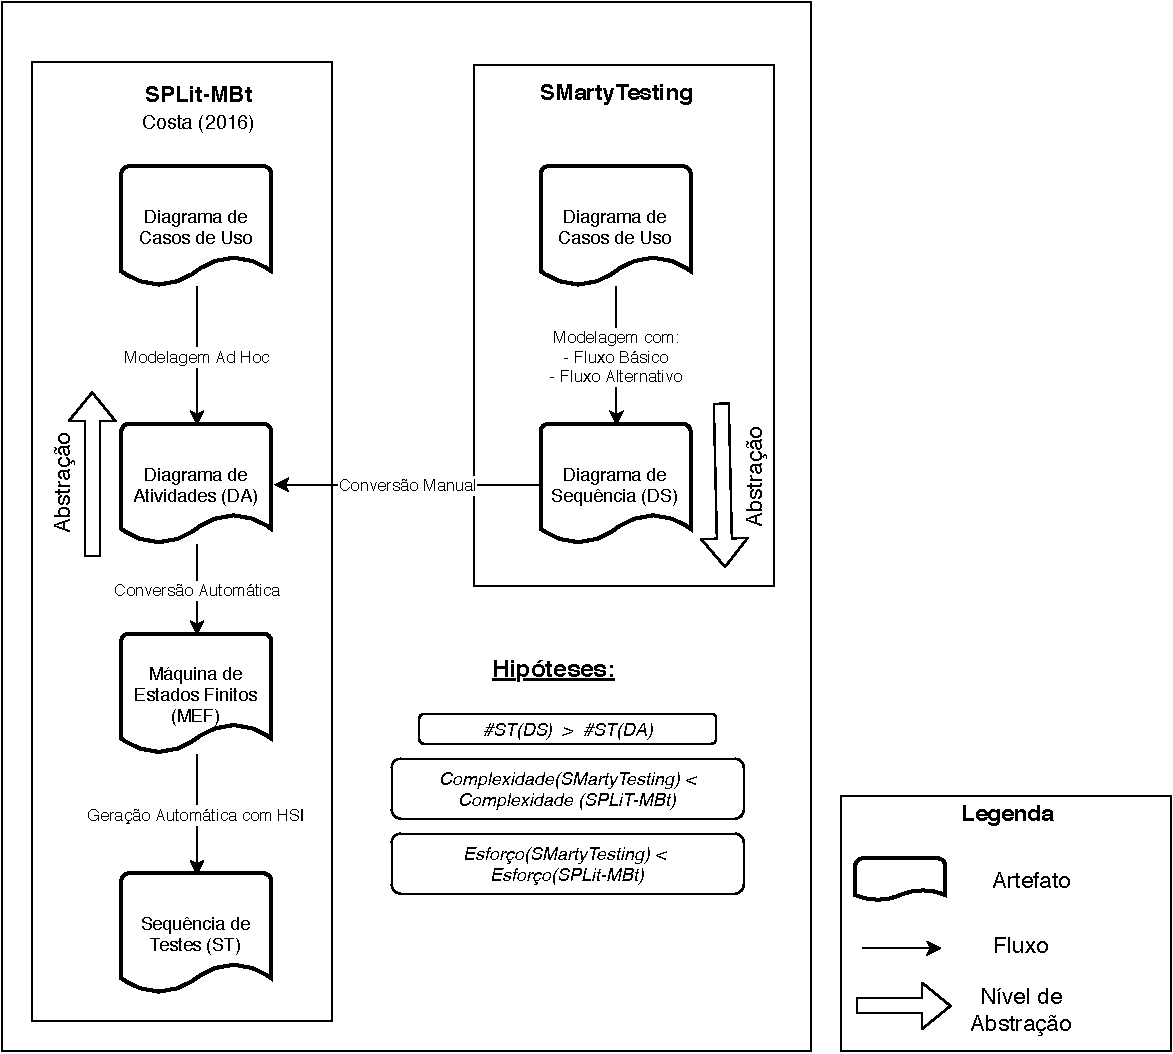
\includegraphics[width=0.85\textwidth]{hipoteses.pdf}
	\caption{Estudo de viabilidade e hipóteses definidas}
	\label{fig:hipoteses}
\end{figure}

\
\subsection{Instrumentação}
Para a geração das sequências de teste foram selecionados três diagramas que contivessem elementos necessários para a validação. A \ref{tab:diagramas_usados} contém as características assim como as variabilidades que cada diagrama possui.
\begin{table}[H]
	\centering
	\caption{Diagramas utilizados no processo de geração de sequências de teste.}
	\label{tab:diagramas_usados}
	\begin{tabular}{l|l|l}
		\hline
		\multicolumn{1}{c|}{\textbf{Modelos}} & \multicolumn{1}{c|}{\textbf{Característica}} & \multicolumn{1}{c}{\textbf{Variabilidade}} \\ \hline
		\begin{tabular}[c]{@{}l@{}}\textbf{\textit{Play Selected Game}}\\ \ref{fig:GamemenuCosta} (DA)\\ \ref{fig:GamemenuKleber} (DS)\end{tabular} & \begin{tabular}[c]{@{}l@{}}\textit{Play Selected Game} é a representação\\ do menu do jogo. Por meio dela é feita\\ a seleção de qual jogo será jogado.\end{tabular} & \begin{tabular}[c]{@{}l@{}}-ponto de variação\\ -variabilidade\\ \textit{-alternative\_OR}\end{tabular} \\ \hline
		\begin{tabular}[c]{@{}l@{}}\textbf{\textit{Save Game}}\\ \ref{fig:SaveGameCosta} (DA)\\ \ref{fig:SaveGameKleber} (DS)\end{tabular} & \textit{Save Game} é a ação de salvar o jogo. & \textit{-mandatory} \\ \hline
		\begin{tabular}[c]{@{}l@{}}\textbf{\textit{Pong Moves}}\\ \ref{fig:pongMovesCosta} (DA)\\ \ref{fig:pong_movesKleber1} (DS)\\\ref{fig:pong_movesKleber2} (DS)\end{tabular} & \begin{tabular}[c]{@{}l@{}}\textit{Pong Moves} são as ações e movimentos\\ do jogo \textit{Pong}.\end{tabular} & - não possui \\ \hline
	\end{tabular}
\end{table}

\subsection{Procedimentos de Análise}

O procedimento de análise segue conforme os critérios definidos na Seção \ref{cap4subsec:criterios}. Porém, para cada critério foi utilizada uma forma de análise diferente, como segue:
\begin{itemize}
	\item \textbf{CT.1:} utilizando comparação de resultados. Quantidade de casos de teste apresentados nas sequências de teste geradas por cada abordagem;
	\item \textbf{CT.2:} utilização de análise de quantidade de caminhos criados por cada geração de sequência. Se uma abordagem gera mais sequências, isso significa que mais caminhos podem ser visitados;
	\item \textbf{CT.3:} para o cálculo de complexidade, foi utilizada a complexidade ciclomática \ref{cap4subsec:ciclomatico}, métrica bastante utilizada para a determinação da quantidade de caminhos seguidos por uma aplicação computacional; e
	\item \textbf{CT.4:} esforço é baseado no tempo de utilização de cada abordagem, em que a abordagem que levar maior tempo para a construção do objetivo final é considerada a de maior esforço de utilização.
\end{itemize}


\section{Execução}
\label{cap4sec:execucaocomparativo}

\subsection{Geração de Sequências de Teste com SPLiT-MBt}
\label{cap4:subsubsec:diagrama_atividade}
Como mencionado anteriormente, foram utilizados três diagramas de atividades que fazem parte da LPS AGM e que foram modelados por \citet{costa2016split}, são eles: \ref{fig:GamemenuCosta}, \ref{fig:SaveGameCosta} e \ref{fig:pongMovesCosta}.

Neste trabalho, cada um deles é acompanhado de uma tabela contendo a sequência de teste gerada por SPLiT-MBt, são elas: \ref{tab:DAGamemenuCosta}, \ref{tab:DASaveGameCosta} e \ref{tab:DApongMovesCosta}. Esses dados serão utilizados na Seção \ref{cap4sec:analiseeinterpretacao} para comparação com diagramas equivalentes aos apresentados por \citet{costa2016split}. 
A \ref{fig:GamemenuCosta} apresenta um diagrama de atividades da LPS AGM que foi utilizado pela SPLiT-MBt para a comparação. 
\newpage
\begin{figure}[H]
	\centering
	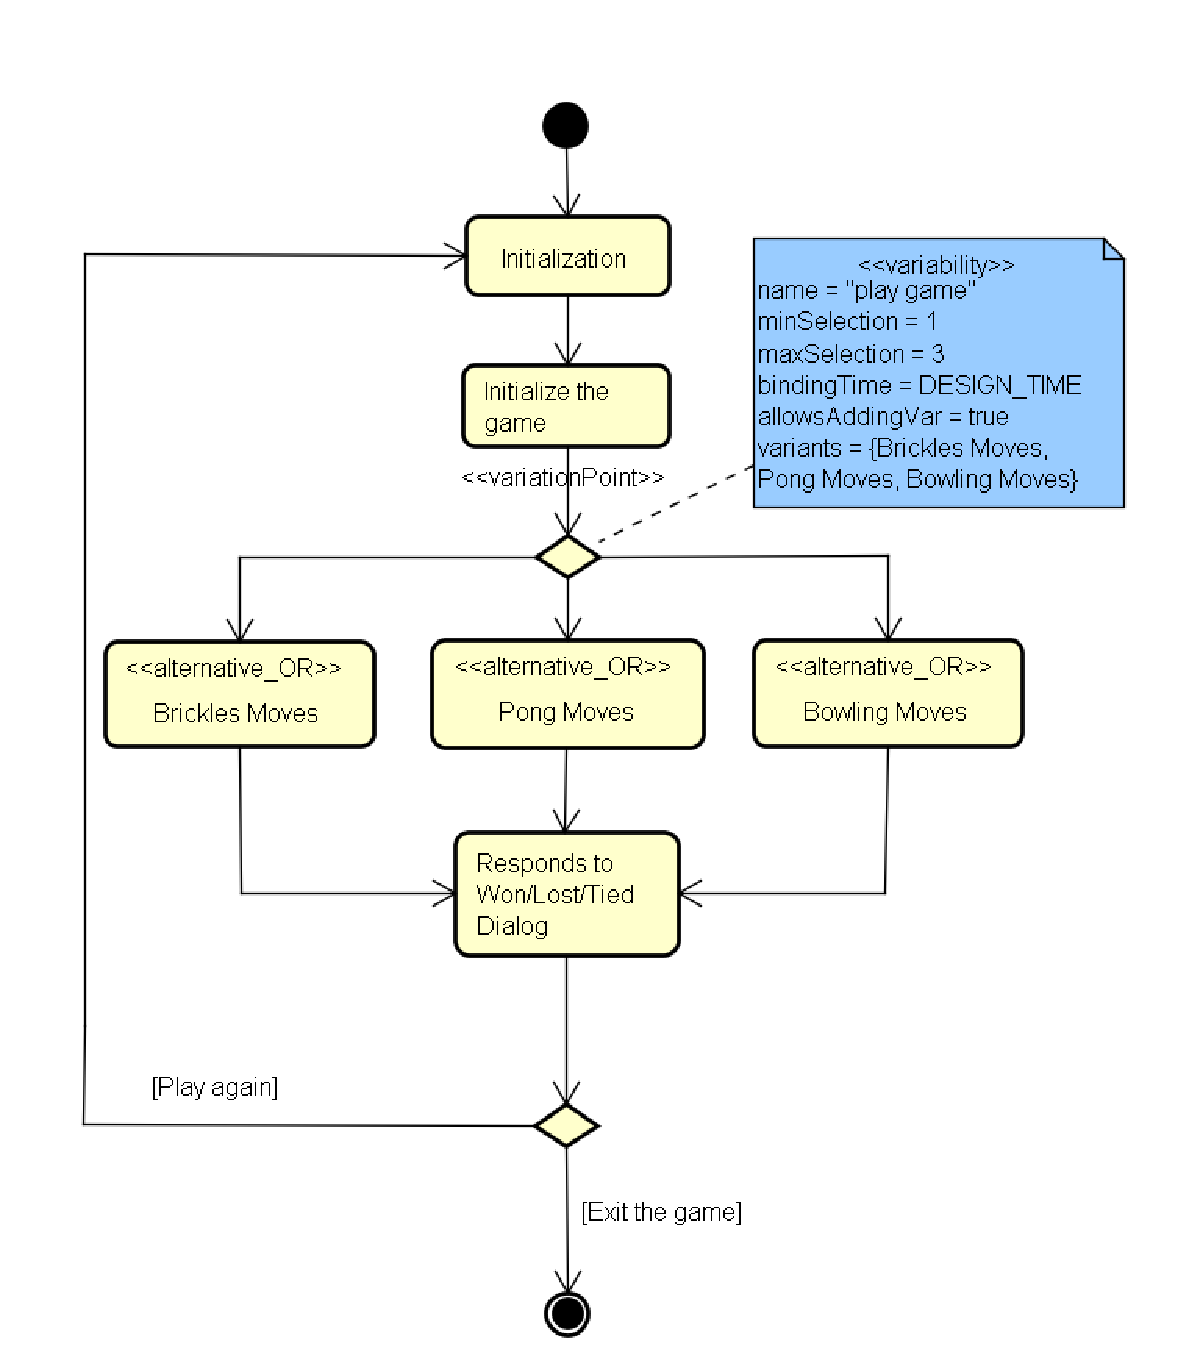
\includegraphics[width=0.75\textwidth]{1_Play_Selected_Game.pdf}
	\caption{Diagrama de Atividades \textit{Play Selected Game} \cite{costa2016split}}
	\label{fig:GamemenuCosta}
\end{figure}

A \ref{tab:DAGamemenuCosta} apresenta os resultados da sequência de teste gerada da \ref{fig:GamemenuCosta}.

%\begin{landscape}
	\begin{table}[H]
		\caption{Sequências de teste do DA \textit{Play Selected Game} da AGM da \ref{fig:GamemenuCosta} gerado por SPLiT-MBt}
		\label{tab:DAGamemenuCosta}
		\footnotesize
		\begin{tabular}{c|c|l|l}
			\hline
			\textbf{\begin{tabular}[c]{@{}c@{}}Sequência \\ de Teste\end{tabular}} & \textbf{Passo} & \textbf{Ação/Descrição} & \textbf{Resultado Esperado} \\ \hline
			\textit{Test Case} 1 & 1 & \begin{tabular}[c]{@{}l@{}}\textit{Initialization}\\ - \textit{Select Play from menu};\end{tabular} & \begin{tabular}[c]{@{}l@{}}Cria as instâncias padrão das\\ classes necessárias.\end{tabular} \\ \hline
			\textit{Test Case} 1 & 2 & \begin{tabular}[c]{@{}l@{}}\textit{Initialize the game}\\ - \textit{Left-click Button to begin play;}\end{tabular} & \begin{tabular}[c]{@{}l@{}}Inicie a ação do jogo e a animação\\começa.\end{tabular} \\ \hline
			\textit{Test Case} 1 & 3 & \begin{tabular}[c]{@{}l@{}}\textit{VP\_Initialize the game}\\ - \{;\\ - b\{\textit{alternative\_OR}\};\\ - c\{\textit{alternative\_OR}\};\\ - a\{\textit{alternative\_OR}\}\};\end{tabular} & \begin{tabular}[c]{@{}l@{}}\{.\\ As pás e o disco começam a se\\mover. \\ A bola começa a se mover. \\ Move a raquete horizontalmente\\para seguir a trilha do mouse \}.\end{tabular} \\ \hline
			\textit{Test Case} 1 & 4 & \begin{tabular}[c]{@{}l@{}}\textit{Responds to Won/Lost/Tied Dialog} \\ - \{;\\ - \textit{Responds to Won/Lost/Tied dialog};\\ - \textit{Responds to Won/Lost/Tied dialog};\\ - \textit{Responds to Won/Lost/Tied dialog} \};\end{tabular} & \begin{tabular}[c]{@{}l@{}}\{.\\ Retorne ao estado inicial do\\ tabuleiro. \\Retorne ao estado inicial do\\tabuleiro. \\A caixa de diálogo para reproduzir\\ novamente é apresentada\}.\end{tabular} \\ \hline
			\textit{Test Case} 1 & 5 & \begin{tabular}[c]{@{}l@{}}\textit{Initialization}\\ - \textit{Respond``yes" in the dialog to play again};\end{tabular} & \begin{tabular}[c]{@{}l@{}}Retorna o tabuleiro de jogo ao seu\\ estado inicializado, pronto para jogar.\end{tabular} \\ \hline
		\end{tabular}
	\end{table}
%\end{landscape}

A \ref{fig:SaveGameCosta} apresenta um diagrama de atividades da LPS AGM que foi utilizado pela SPLiT-MBt para a comparação. 

\begin{figure}[H]
	\centering
	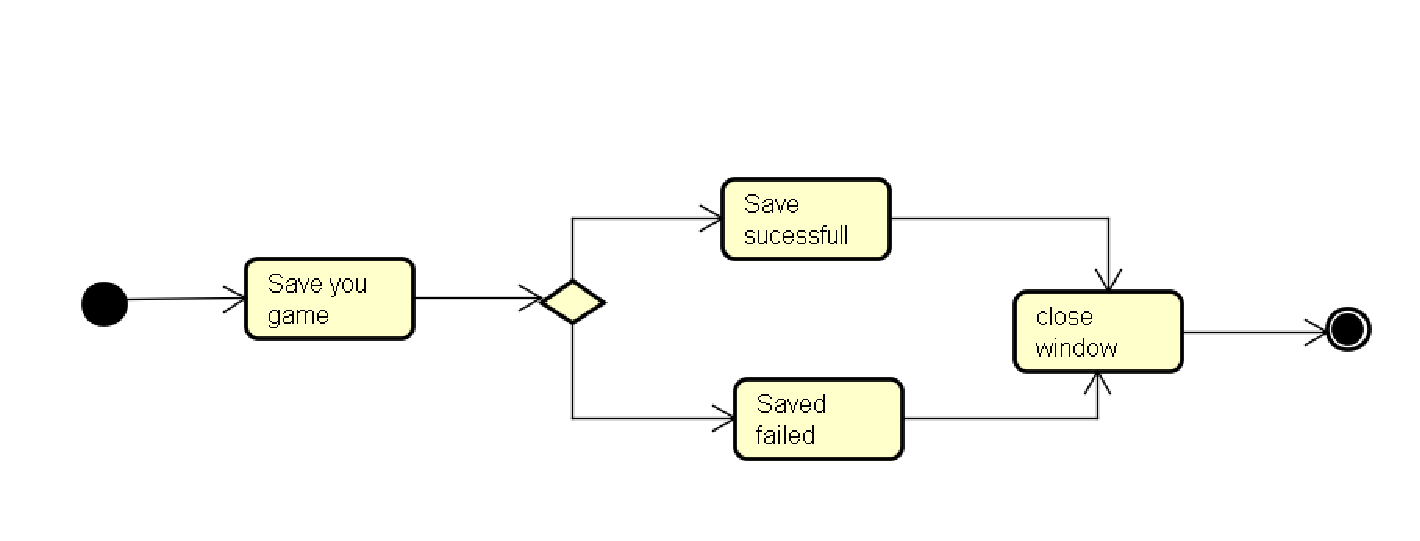
\includegraphics[width=\textwidth]{2_Save_Game.pdf}
	\caption{Diagrama de Atividades \textit{Save Game} \cite{costa2016split}}
	\label{fig:SaveGameCosta}
\end{figure}
\newpage
A \ref{tab:DASaveGameCosta} apresenta os resultados da sequência de teste gerada da \ref{fig:SaveGameCosta}.

	\begin{table}[H]
		\caption{Sequências de teste do DA \textit{Save Game} da \ref{fig:SaveGameCosta} geradas por SPLiT-MBt}
		\label{tab:DASaveGameCosta}
		\begin{tabular}{p{2.5cm}|p{1cm}|p{6cm}|p{5cm}}
			\hline
			\textbf{\begin{tabular}[c]{@{}c@{}}Sequência \\ de Teste\end{tabular}} & \textbf{Passo} & \textbf{Ação/Descrição} & \textbf{Resultado Esperado} \\ \hline
			\textit{Test Case} 1 & 1 & \begin{tabular}[c]{@{}l@{}}\textit{Save your game}\\ - \textit{save GAME window are showed};\end{tabular} & Termine o jogo. \\ \hline
			\textit{Test Case} 1 & 2 & \begin{tabular}[c]{@{}l@{}}\textit{Saved failed}\\ - \textit{click SAVE GAME  button};\end{tabular} & mensagem SALVAR JOGO com falha é mostrada. \\ \hline
			\textit{Test Case} 1 & 3 & \begin{tabular}[c]{@{}l@{}}\textit{close window}\\ - \textit{Click close SAVE THE GAME};\end{tabular} & A janela SALVAR JOGO é fechada. \\ \hline
			\textit{Test Case} 2 & 1 & \begin{tabular}[c]{@{}l@{}}\textit{Save your game}\\ - \textit{save GAME window are showed};\end{tabular} & Termine o jogo. \\ \hline
			\textit{Test Case} 2 & 2 & \begin{tabular}[c]{@{}l@{}}\textit{Save sucessfull}\\ - \textit{click SAVE GAME button};\end{tabular} & messagem SALVAR JOGO é mostrada. \\ \hline
			\textit{Test Case} 2 & 3 & \begin{tabular}[c]{@{}l@{}}\textit{close window}\\ - \textit{click close SAVE GAME button};\end{tabular} & A janela SALVAR JOGO é fechada. \\ \hline
		\end{tabular}
	\end{table}

A \ref{fig:pongMovesCosta} apresenta um diagrama de atividades da LPS AGM que foi utilizado pela SPLiT-MBt para a comparação.

\begin{figure}[H]
	\centering
	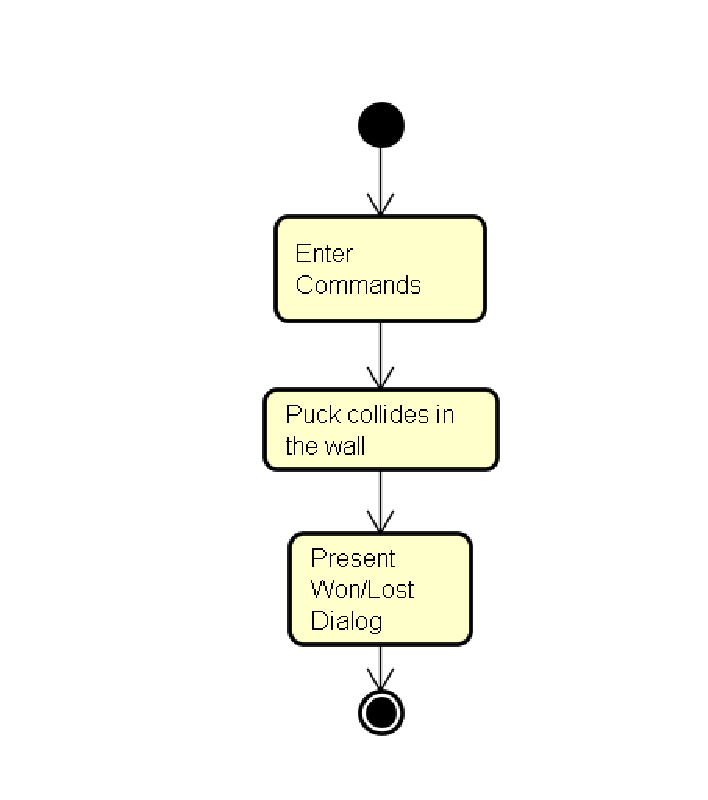
\includegraphics[width=0.2\textwidth]{3_pong_Moves.pdf}
	\caption{Diagrama de Atividades \textit{Pong Moves} \cite{costa2016split}}
	\label{fig:pongMovesCosta}
\end{figure}
\newpage
A \ref{tab:DApongMovesCosta} apresenta os resultados da sequência de teste gerada da \ref{fig:pongMovesCosta}.

	\begin{table}[H]
		\caption{Sequencia de teste do DA \textit{Pong Moves} da \ref{fig:pongMovesCosta} gerada por SPLiT-MBt}
		\label{tab:DApongMovesCosta}
		\begin{tabular}{p{2.5cm}|p{1cm}|p{5.5cm}|p{6cm}}
			\hline
			\textbf{\begin{tabular}[c]{@{}c@{}}Sequência \\ de Teste\end{tabular}} & \textbf{Passo} & \textbf{Ação/Descrição} & \textbf{Resultado Esperado} \\ \hline
			\textit{Test Case} 1 & 1 & \begin{tabular}[c]{@{}l@{}}\textit{Enter Commands}\\ - \textit{Pong};\end{tabular} & Disco começa a se mover. \\ \hline
			\textit{Test Case} 1 & 2 & \begin{tabular}[c]{@{}l@{}}\textit{Puck collides in the wall}\\ - \textit{Let the puck collide into} \\ \textit{the walls};\end{tabular} & \begin{tabular}[c]{@{}l@{}}Com base nas regras, o disco é \\ absorvido ou muda de direção \\ de acordo com as leis da física.\end{tabular} \\ \hline
			\textit{Test Case} 1 & 3 & \begin{tabular}[c]{@{}l@{}}\textit{Present Won/Lost Dialog} \\ - \textit{The puck is absorbed by the} \\ \textit{left or right side of the playing} \\ \textit{field};\end{tabular} & A caixa de diálogo Ganhos / Perdas é apresentada. \\ \hline
		\end{tabular}
	\end{table}

\newpage

\subsection{Geração de Sequências de Teste com \textit{SMartyTesting}}
\label{cap4subsubsec:diagrama_sequencia}

Após a geração da sequência de teste com DA como artefatos de entrada da SPLiT-MBt, são utilizados DS criados por \citet{marcolino2017variability}, equivalentes aos DA criados por \citet{costa2016split} que são os da \ref{fig:GamemenuKleber}, \ref{fig:SaveGameKleber} e \ref{fig:pong_movesKleber1}.


Essa equivalência se deve ao fato do nível de abstração utilizado, um exemplo é a \ref{fig:SaveGameCosta} que representa o \textit{Save Game}, nela são observadas duas condições, onde houve sucesso e onde houve falha no salvamento. Nesse caso, a representação em DS por ser mais próxima ao código dar-se-ia em dois diagramas: um para sucesso e outro para falha. A \ref{fig:SaveGameKleber} representa somente a condição de sucesso.   

Após essa criação, os DS foram utilizados em \textit{SMartyTesting} para a geração de sequências de teste para comparação. Na etapa inicial foi realizada a conversão para DA conforme pode ser visto nas figuras: \ref{fig:GamemenuKleberDStoDA}, \ref{fig:SaveGameKleberDStoDA} e \ref{fig:pong_movesDS_to_DA1}, que na etapa seguinte foram utilizados para a geração das sequências de teste: \ref{tab:GamemenuKleberDStoDA}, \ref{tab:SaveGameKleberDStoDA} e \ref{tab:pong_movesDS_to_DA}.

A \ref{fig:GamemenuKleber} apresenta um diagrama de sequência da LPS AGM que foi utilizado por \textit{SMartyTesting} para a conversão para DA.

%\begin{landscape}
	\begin{figure}[H]
		\centering
		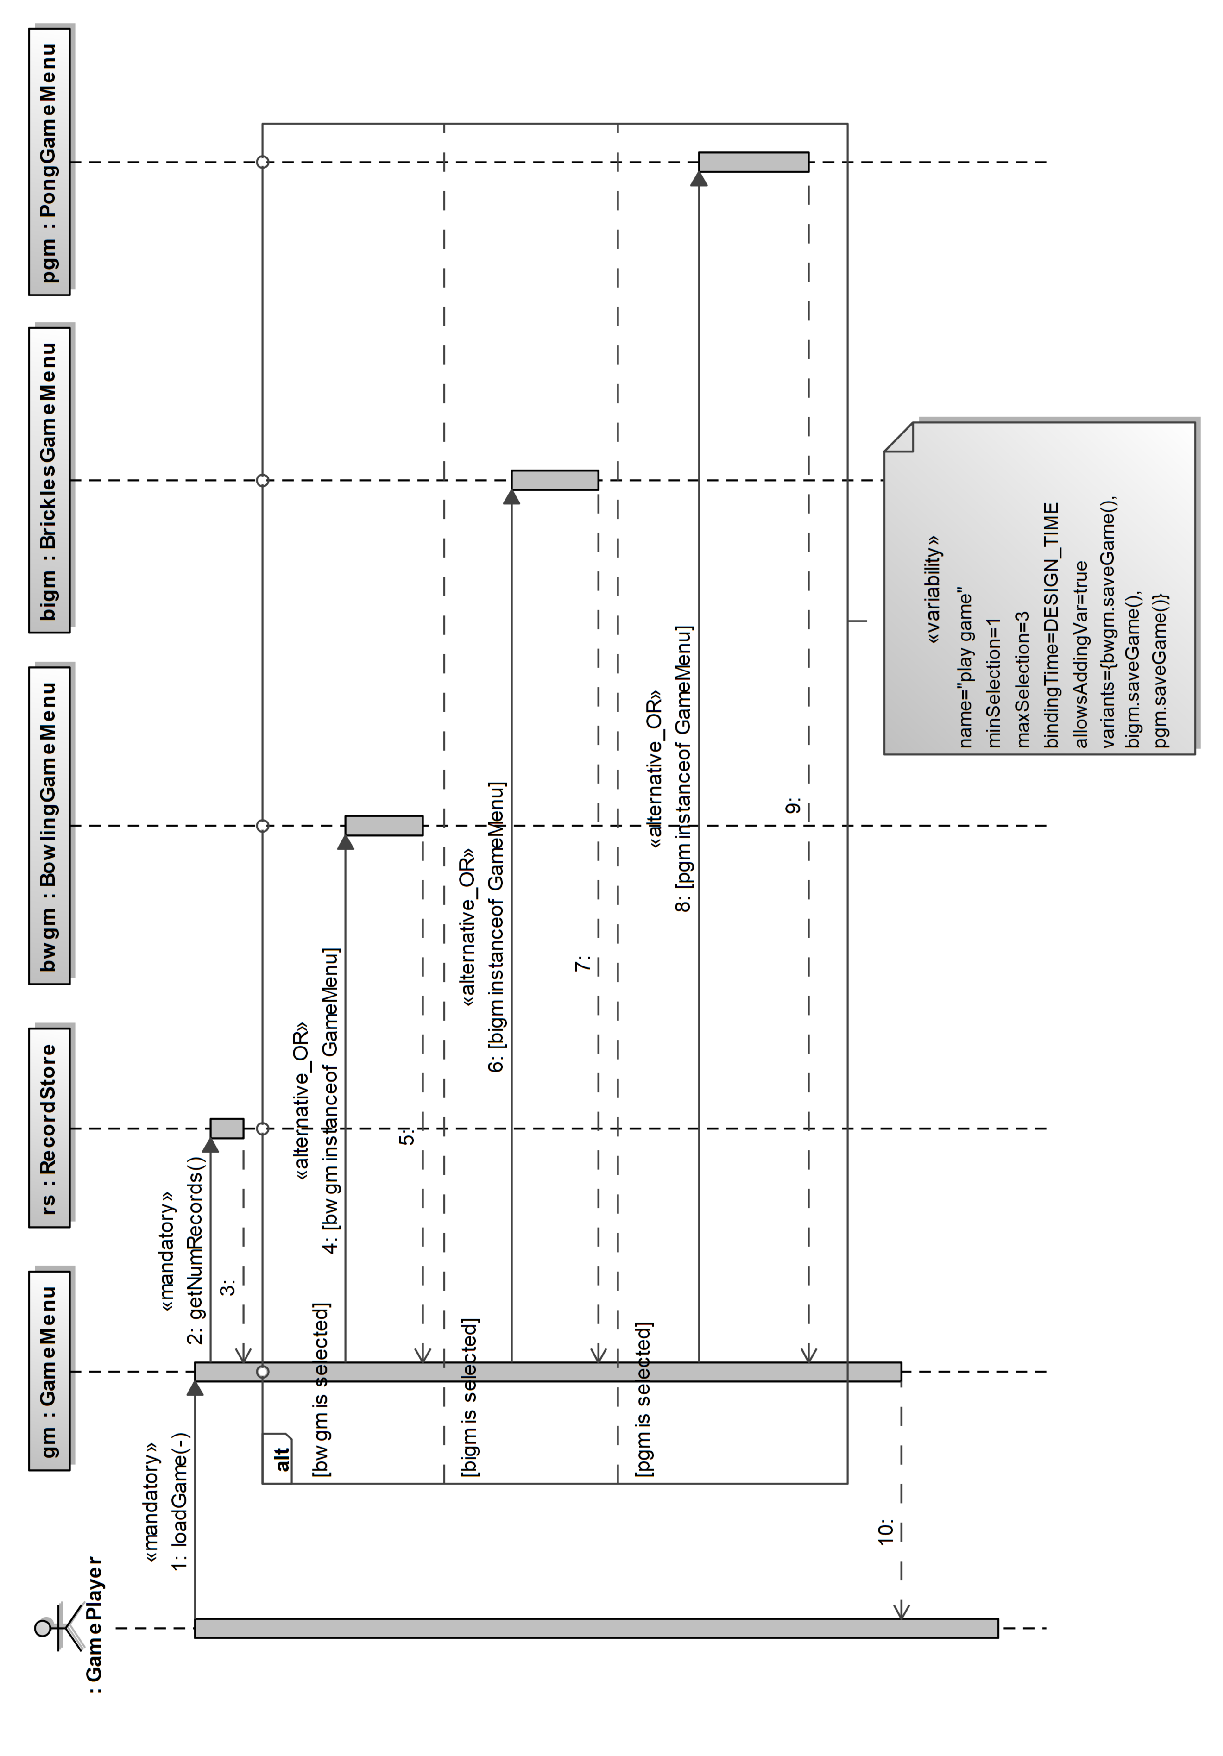
\includegraphics[width=0.75\textwidth]{1_loadGame_LP_View2.pdf}
		\caption{Diagrama de Sequência \textit{Play Selected Game} \cite{marcolino2017variability}}
		\label{fig:GamemenuKleber}
	\end{figure}
%\end{landscape}

A \ref{fig:GamemenuKleberDStoDA} apresenta um diagrama de atividades da LPS AGM que foi convertido por \textit{SMartyTesting} para a geração de sequências de teste.

%\begin{landscape}
	\begin{figure}[H]
		\centering
		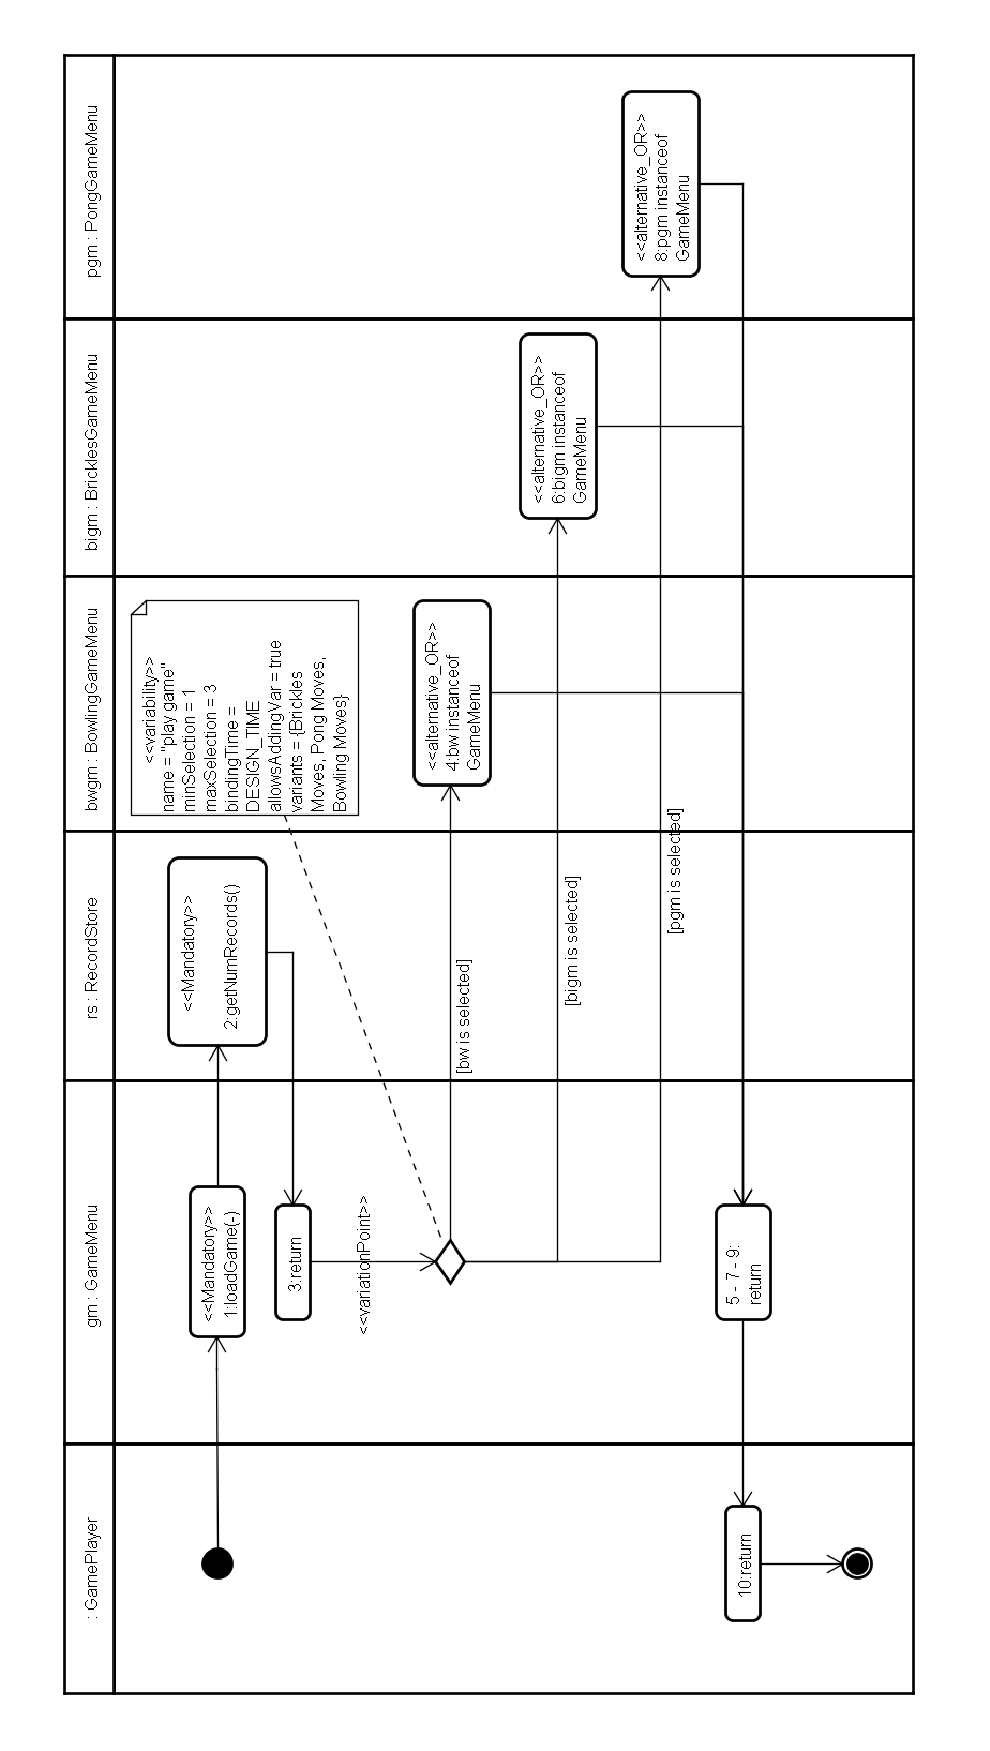
\includegraphics[width=0.63\textwidth]{1_Play_Selected_Game_DS_to_DA2.pdf}
		\caption{Diagrama de Atividades resultantes do Diagrama de Sequência da \ref{fig:GamemenuKleber}}
		\label{fig:GamemenuKleberDStoDA}
	\end{figure}
%\end{landscape}

A \ref{tab:GamemenuKleberDStoDA} apresenta os resultados da sequência de teste gerada da \ref{fig:GamemenuKleberDStoDA}.

%\begin{landscape}
	\begin{table}[H]
		\caption{Sequências de casos de teste DA da \ref{fig:GamemenuKleberDStoDA} geradas por \textit{SMartyTesting}}
		\label{tab:GamemenuKleberDStoDA}
		\footnotesize
		\begin{tabular}{c|c|l|l}
			\hline
			\textbf{\begin{tabular}[c]{@{}c@{}}Sequência \\ de Teste\end{tabular}} & \textbf{Passo} & \textbf{Ação/Descrição} & \textbf{Resultado Esperado} \\ \hline
			\textit{Test Case} 1 & 1 & \begin{tabular}[c]{@{}l@{}}1:\textit{loadGame}(-)\\ - \textit{Game Player} dispara método \\ \textit{loadGame}\{\textit{Mandatory}\};\end{tabular} & \textit{loadGame} é carregado. \\ \hline
			\textit{Test Case} 1 & 2 & \begin{tabular}[c]{@{}l@{}}2:\textit{getNumRecords}()\\ - \textit{Game menu} após carregado faz \\ uso do método \textit{getNumRecords}\{\textit{Mandatory}\};\end{tabular} & acessa dados de \textit{recordStore}. \\ \hline
			\textit{Test Case} 1 & 3 & \begin{tabular}[c]{@{}l@{}}3:\textit{return}\\ - \textit{recordStore} envia mensagens de retorno;\end{tabular} & \begin{tabular}[c]{@{}l@{}}Dados de pontuação são\\ retornados por\\ \textit{getNumrecords} para \textit{GameMenu}.\end{tabular} \\ \hline
			\textit{Test Case} 1 & 4 & \begin{tabular}[c]{@{}l@{}}VP\_3:\textit{return}\\ - \{;\\ - Opção bw é selecionada\{\textit{alternative\_OR\}};\\ - Opção bigm é selecionada\{\textit{alternative\_OR\}};\\ - Opção pgm é selecionada\{\textit{alternative\_OR\}}\};\end{tabular} & \begin{tabular}[c]{@{}l@{}}\{.\\ Instancia recurso da opção\\ \textit{bowling}.\\ instancia recurso da opção\\ bigm \textit{brickles}.\\ instancia recurso da opção\\ \textit{pong}\}.\end{tabular} \\ \hline
			\textit{Test Case} 1 & 5 & \begin{tabular}[c]{@{}l@{}}5 - 7 - 9:\textit{return}\\ - \{;\\ - Retorno da opção bw;\\ - Retorno da opção bigm;\\ - Retorno da opção pgm\};\end{tabular} & \begin{tabular}[c]{@{}l@{}}\{.\\ Retorna após bw \textit{instanceof}\\ \textit{GameMenu} for executada.\\ Retorna após bigm \textit{instanceof}\\ GameMenu for executada.\\ Retorna após pgm \textit{instanceof}\\ \textit{GameMenu} for executada\}.\end{tabular} \\ \hline
			\textit{Test Case} 1 & 6 & \begin{tabular}[c]{@{}l@{}}10:\textit{return}\\ - Retorno da informação ao \textit{Game Player};\end{tabular} & \begin{tabular}[c]{@{}l@{}}\textit{Player} recebe retorno da ação\\ escolhida.\end{tabular} \\ \hline
		\end{tabular}
	\end{table}
%\end{landscape}

A \ref{fig:SaveGameKleber} apresenta um diagrama de sequência da LPS AGM que foi utilizado por \textit{SMartyTesting} para a conversão para DA.

\begin{landscape}
	\begin{figure}[H]
		\centering
		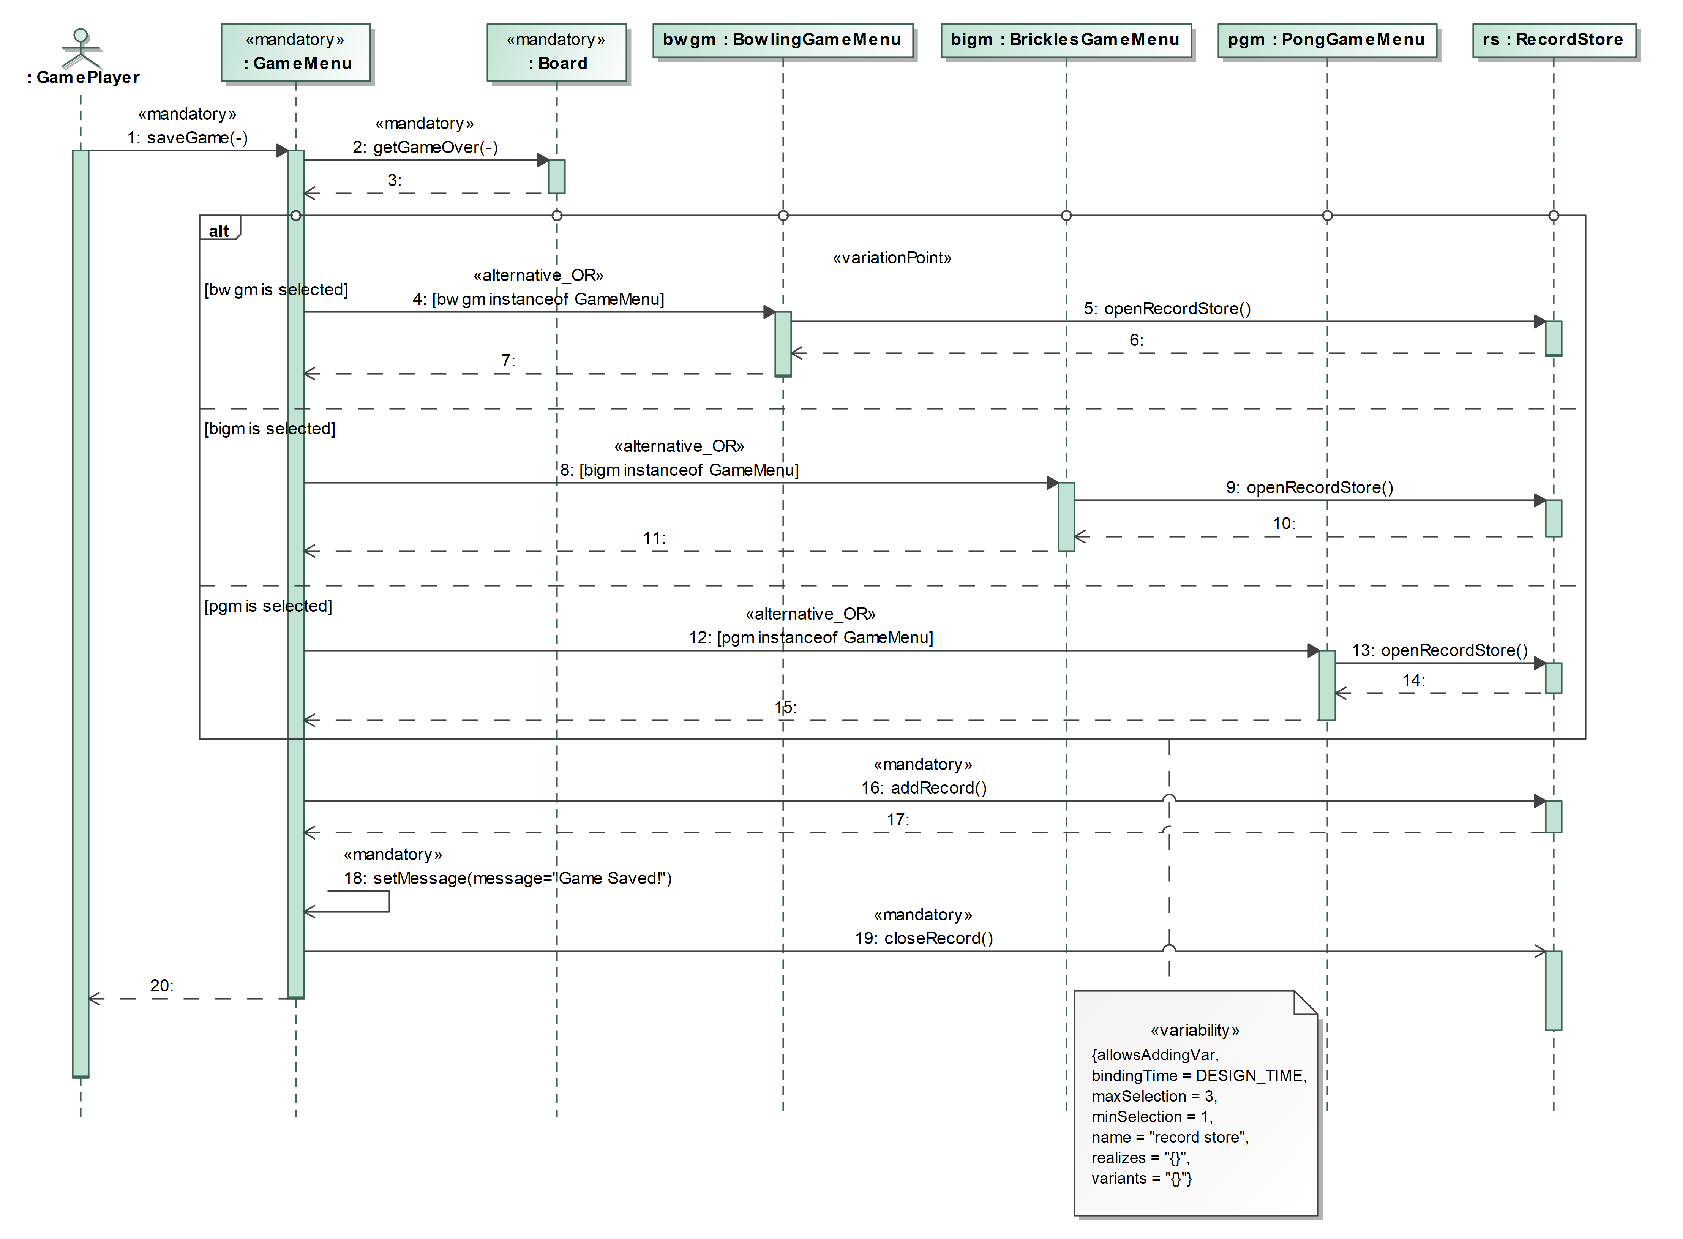
\includegraphics[scale=0.70]{2_saveGame_LP_View.pdf}
		\caption{Diagrama de Sequência \textit{Save Game} \cite{marcolino2017variability}}
		\label{fig:SaveGameKleber}
	\end{figure}
\end{landscape}

A \ref{fig:SaveGameKleberDStoDA} apresenta um diagrama de atividades da LPS AGM que foi convertido por \textit{SMartyTesting} para a geração de sequências de teste.

%\begin{landscape}
	\begin{figure}[H]
		\centering
		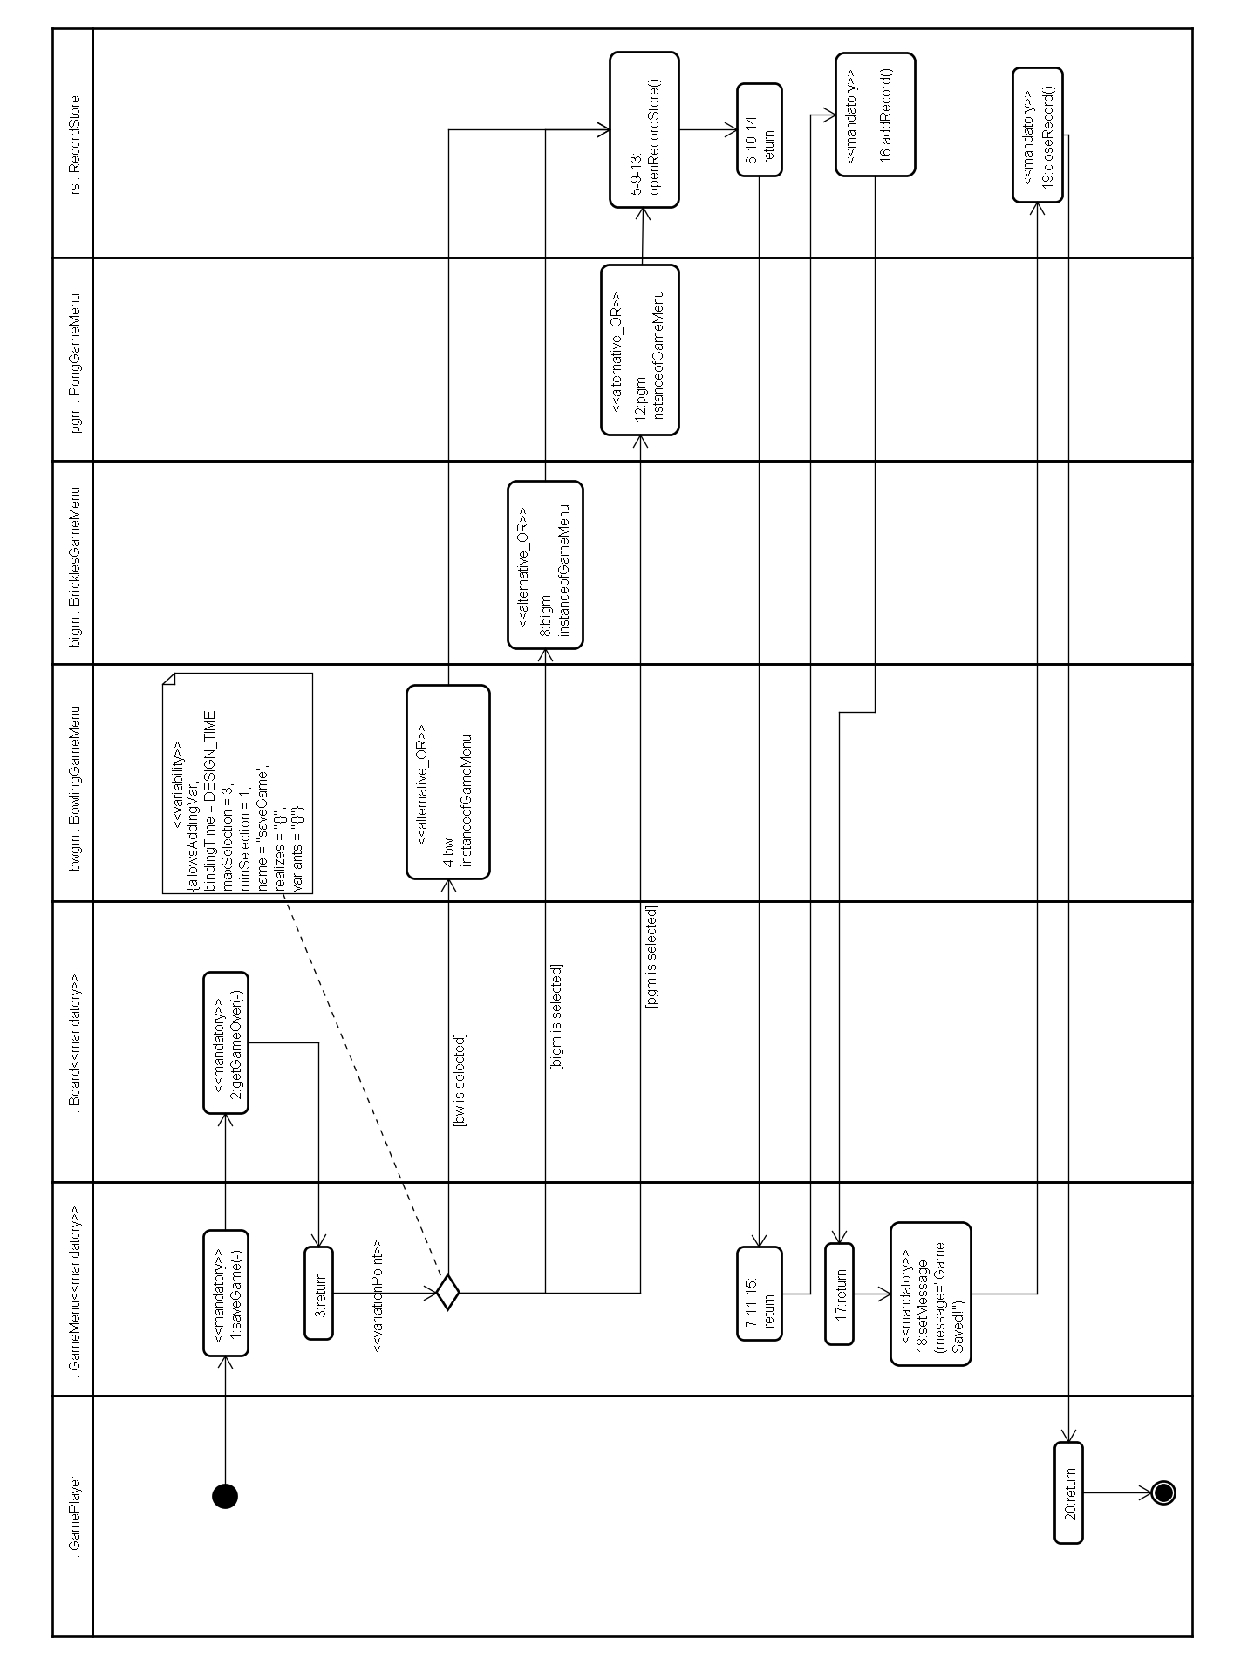
\includegraphics[width=0.8\textwidth]{2_saveGame_LP_View_DS_to_DA2.pdf}
		\caption{Diagrama de Atividades resultante dos Diagrama de Sequência da \ref{fig:SaveGameKleber}}
		\label{fig:SaveGameKleberDStoDA}
	\end{figure}
%\end{landscape}

A \ref{tab:SaveGameKleberDStoDA} apresenta os resultados da sequência de teste gerada da \ref{fig:SaveGameKleberDStoDA}.

\begin{landscape}
	\begin{table}[h!]
		\caption{Sequências de teste DA da \ref{fig:SaveGameKleberDStoDA} geradas por \textit{SMartyTesting}}
		\label{tab:SaveGameKleberDStoDA}
		\begin{tabular}{c|c|l|l}
			\hline
			\textbf{\begin{tabular}[c]{@{}c@{}}Sequência \\ de Teste\end{tabular}} & \textbf{Passo} & \textbf{Ação/Descrição} & \textbf{Resultado Esperado} \\ \hline
			\textit{Test Case} 1 & 1 & \begin{tabular}[c]{@{}l@{}}1:\textit{saveGame}(-)\\ - \textit{GamePlayer} dispara método \\ \textit{saveGame}\{\textit{mandatory}\};\end{tabular} & \textit{GameMenu} é carregado. \\ \hline
			\textit{Test Case} 1 & 2 & \begin{tabular}[c]{@{}l@{}}2:\textit{getGameOver}(-)\\ - \textit{GameMenu} dispara método \\ \textit{getGameOver}\{\textit{mandatory}\};\end{tabular} & \textit{Board} verifica ação. \\ \hline
			\textit{Test Case} 1 & 3 & \begin{tabular}[c]{@{}l@{}}3:\textit{return}\\ - \textit{Board} retorna solicitação;\end{tabular} & Valor retorna para jogo selecionado. \\ \hline
			\textit{Test Case} 1 & 4 & \begin{tabular}[c]{@{}l@{}}VP\_3:\textit{return}\\ - \{; bw é selecionado\{\textit{alternative\_OR}\};\\ - bigm é selecionado\{\textit{alternative\_OR}\};\\ - pgm é selecionado\{\textit{alternative\_OR}\}\};\end{tabular} & \begin{tabular}[c]{@{}l@{}}\{.\\ dispara método \textit{instanceofGameMenu}.\\ dispara método \textit{instanceofGameMenu}.\\ dispara método \textit{instanceofGameMenu}\}.\end{tabular} \\ \hline
			\textit{Test Case} 1 & 5 & \begin{tabular}[c]{@{}l@{}}5-9-13:\textit{openRecordStore}()\\ - \{; bw envia dados para método \textit{openRecordStore};\\ - bigm envia dados para método \textit{openRecordStore};\\ - pgm envia dados para método \textit{openRecordStore}\};\end{tabular} & \begin{tabular}[c]{@{}l@{}}\{.\\ dados são utilizados por \textit{openRecordStore}.\\ dados são utilizados por \textit{openRecordStore}.\\ dados são utilizados por \textit{openRecordStore}\}.\end{tabular} \\ \hline
			\textit{Test Case} 1 & 6 & \begin{tabular}[c]{@{}l@{}}6-10-14:\textit{return}\\ - \textit{operRecordStore} retorna para bw - bigm - pgm;\end{tabular} & confirma se possui dados disponíveis. \\ \hline
			\textit{Test Case} 1 & 7 & \begin{tabular}[c]{@{}l@{}}7-11-15:\textit{return}\\ - Return dos dados para \textit{GameMenu};\end{tabular} & \begin{tabular}[c]{@{}l@{}}dados disponíveis são retornados \\ para serem adicionados.\end{tabular} \\ \hline
			\textit{Test Case} 1 & 8 & \begin{tabular}[c]{@{}l@{}}16:\textit{addRecord}()\\ - acionado método \textit{addRecord}\{\textit{mandatory}\};\end{tabular} & Dados são salvos. \\ \hline
			\textit{Test Case} 1 & 9 & \begin{tabular}[c]{@{}l@{}}17:\textit{return}\\ - retorna ação do \textit{addRecord};\end{tabular} & Confirma persistência dos dados. \\ \hline
			\textit{Test Case} 1 & 10 & \begin{tabular}[c]{@{}l@{}}18:\textit{setMessage(message="Game Saved!")}\\ - dispara mensagem de confirmação\{\textit{mandatory}\};\end{tabular} & Mensagem de confirmação apresentada. \\ \hline
			\textit{Test Case} 1 & 11 & \begin{tabular}[c]{@{}l@{}}19:\textit{closeRecord}()\\ - Dispara método \textit{closeRecord}\{\textit{mandatory}\};\end{tabular} & Método encerra operação. \\ \hline
			\textit{Test Case} 1 & 12 & \begin{tabular}[c]{@{}l@{}}20:\textit{return}\\ - retornar confirmação da operação;\end{tabular} & \begin{tabular}[c]{@{}l@{}}Concluída com sucesso devolver \\ Confirmação ao usuário\end{tabular} \\ \hline
		\end{tabular}
	\end{table}
\end{landscape}

A \ref{fig:pong_movesKleber1} e a \ref{fig:pong_movesKleber2} apresentam um diagrama de sequência da LPS AGM que foi utilizado por \textit{SMartyTesting} para a conversão para DA.

%\begin{landscape}
	\begin{figure}[H]
		\centering
		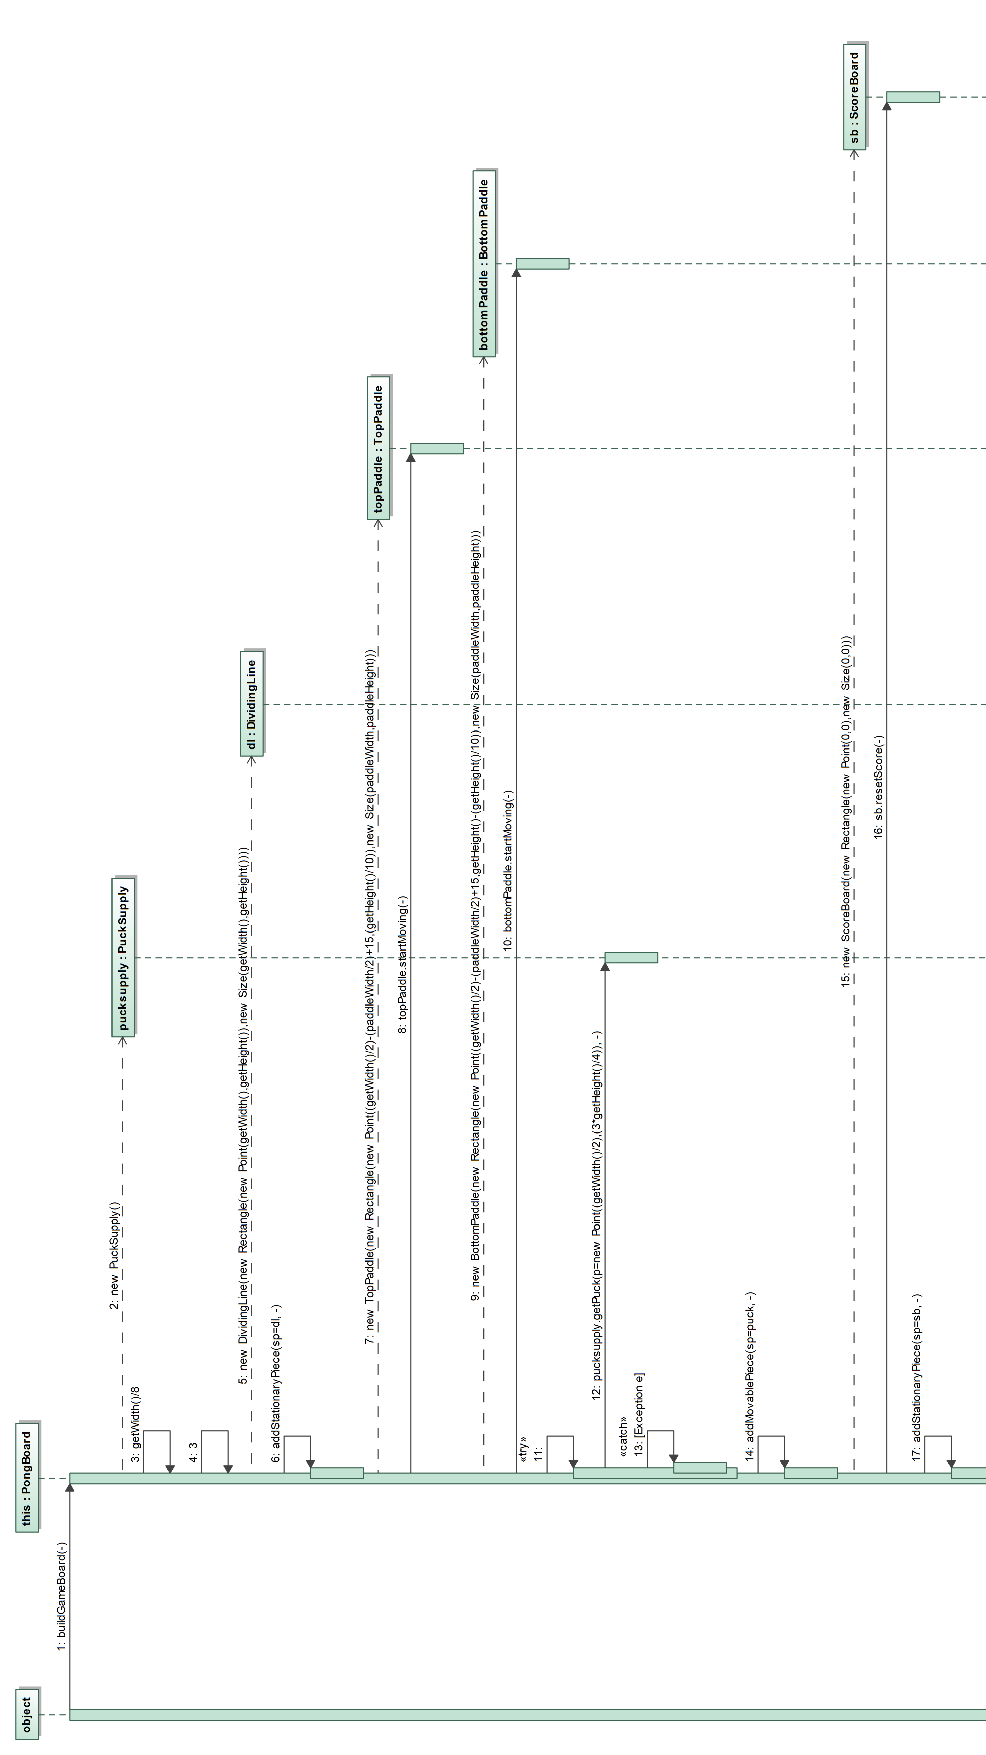
\includegraphics[width=0.7\textwidth]{3_DS_pong_moves_1_2.pdf}
		\caption{Diagrama de Sequência \textit{Pong Moves} 1 \cite{marcolino2017variability}}
		\label{fig:pong_movesKleber1}
	\end{figure}
%\end{landscape}

\begin{landscape}
	\begin{figure}[H]
		\centering
		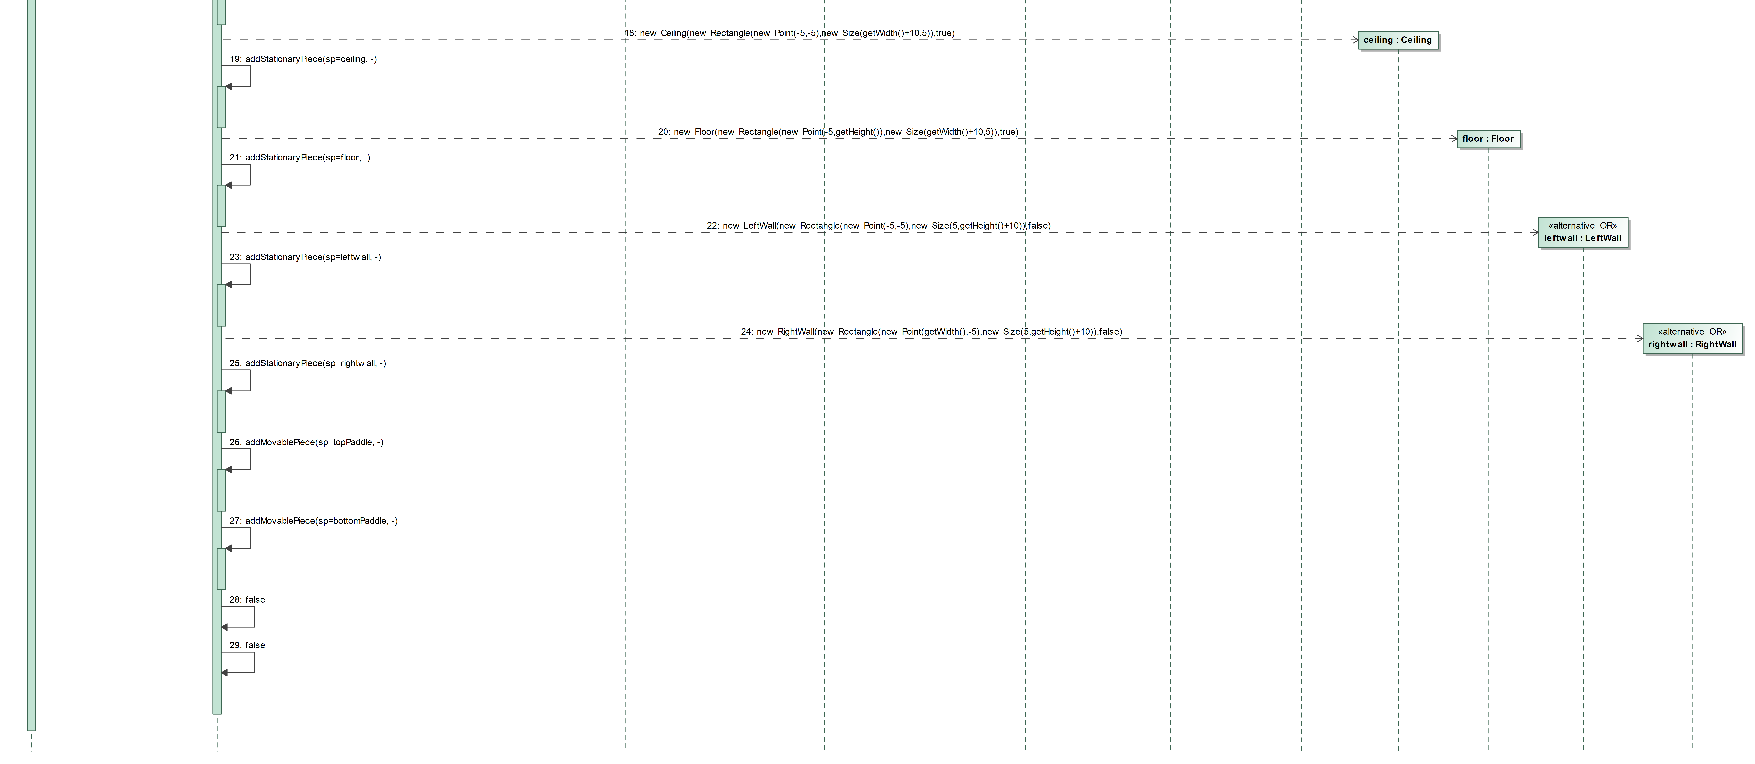
\includegraphics[scale=0.75]{3_DS_pong_moves_2.pdf}
		\caption{Diagramas de Sequência \textit{Pong Moves} 2 \cite{marcolino2017variability}}
		\label{fig:pong_movesKleber2}
	\end{figure}
\end{landscape}

As \ref{fig:pong_movesDS_to_DA1} e \ref{fig:pong_movesDS_to_DA2} apresentam um diagrama de atividades da LPS AGM que foi convertido por \textit{SMartyTesting} para a geração de sequências de teste.

A \ref{tab:pong_movesDS_to_DA} apresenta os resultados da sequência de teste gerada das \ref{fig:pong_movesDS_to_DA1} e \ref{fig:pong_movesDS_to_DA2}

%\begin{landscape}
	\begin{figure}[H]
		\centering
		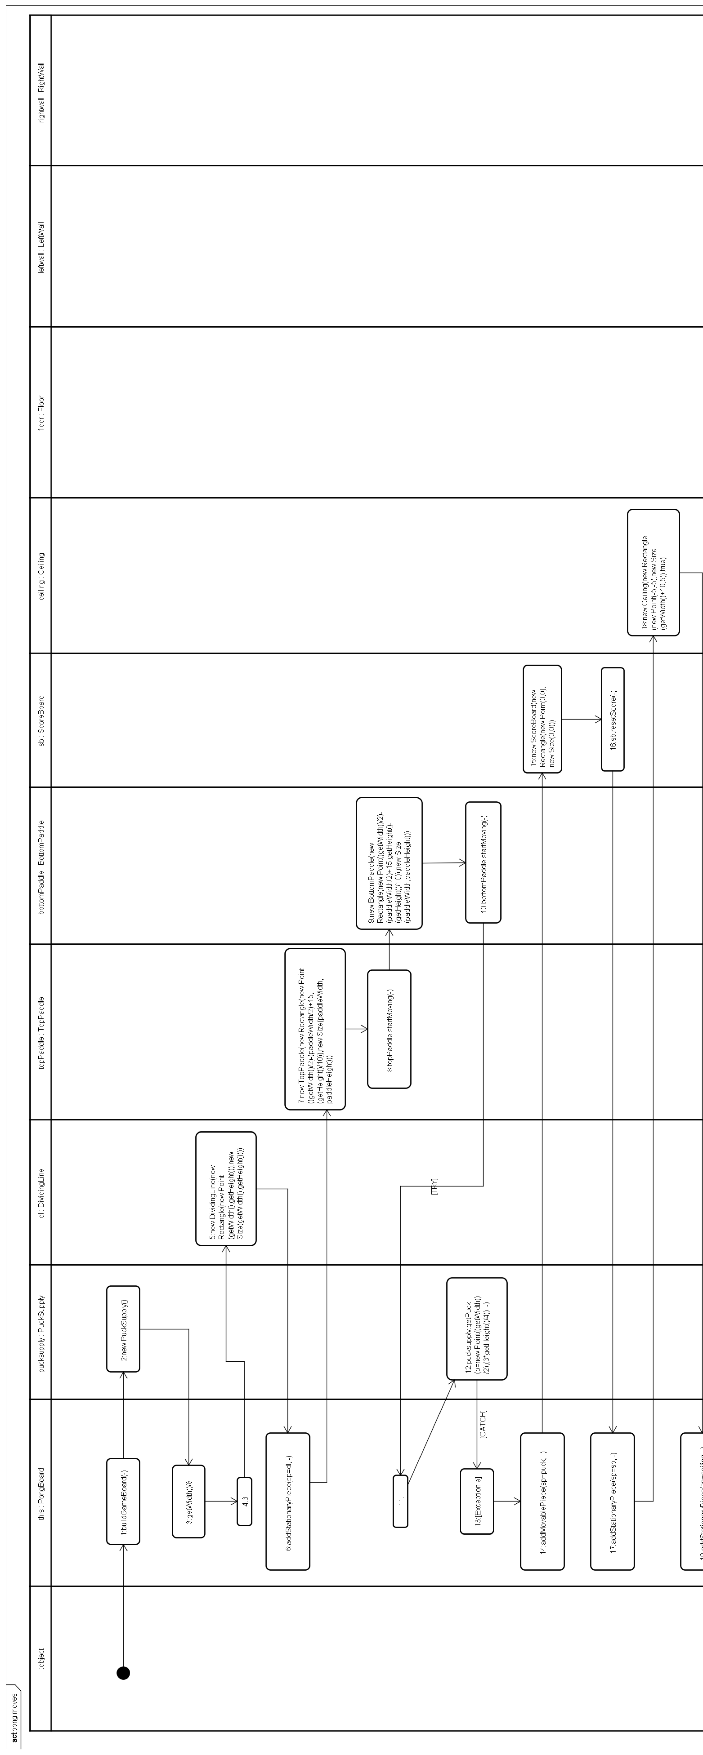
\includegraphics[scale=0.61]{3_pong_moves_DS_to_DA1.pdf}
		\caption{Diagrama de Atividades resultante do Diagrama de Sequência da \ref{fig:pong_movesKleber1} e da \ref{fig:pong_movesKleber2} parte 1}
		\label{fig:pong_movesDS_to_DA1}
	\end{figure}
%\end{landscape}
\begin{landscape}
	\begin{figure}[H]
		\centering
		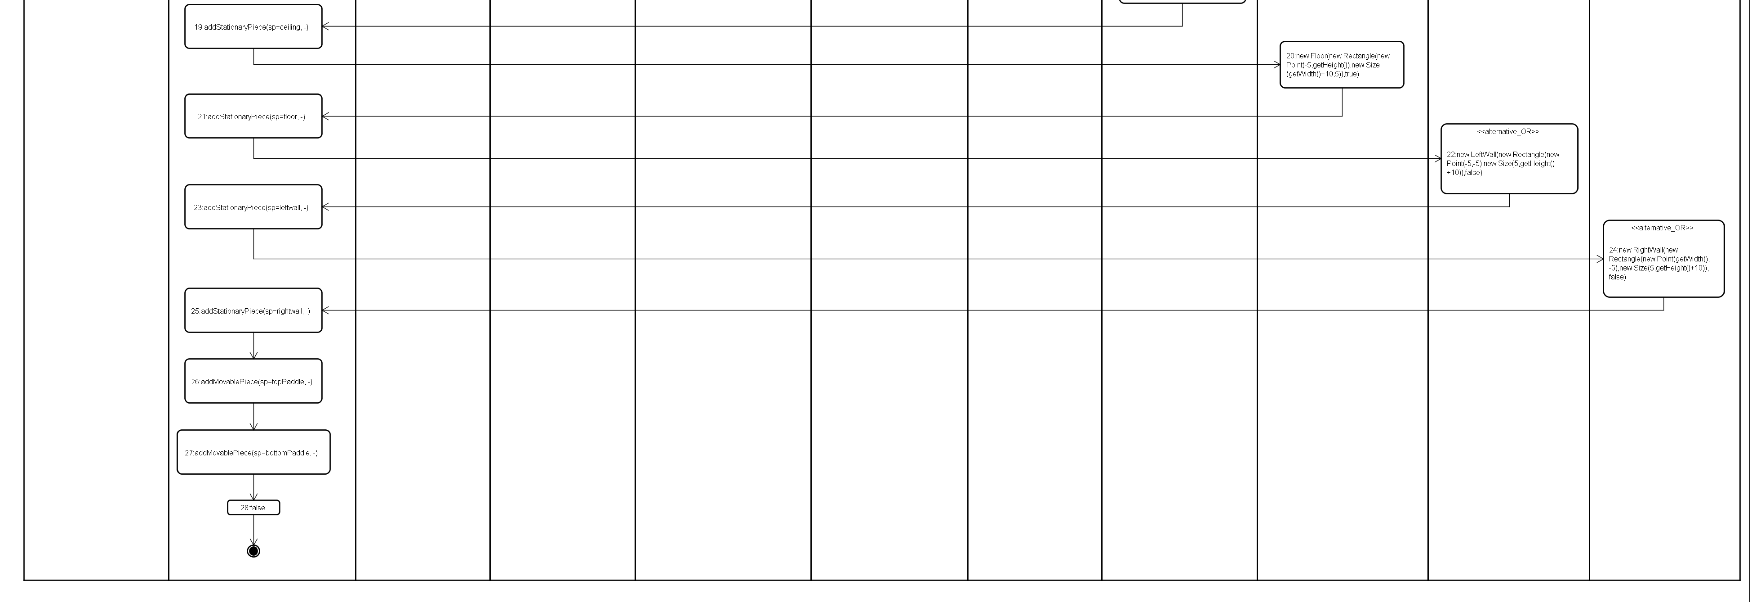
\includegraphics[scale=0.70]{3_pong_moves_DS_to_DA2.pdf}
		\caption{Diagrama de Atividades resultante do Diagrama de Sequência da \ref{fig:pong_movesKleber1} e da \ref{fig:pong_movesKleber2} parte 2}
		\label{fig:pong_movesDS_to_DA2}
	\end{figure}
\end{landscape}
%\end{landscape}



\begin{landscape}
	\begin{longtable}{c|c|l|l}
		\caption{Sequências de teste do DA da \ref{fig:pong_movesDS_to_DA1} geradas por \textit{SMartyTesting}}
		\label{tab:pong_movesDS_to_DA}\\
		\hline
		\textbf{\begin{tabular}[c]{@{}c@{}}Sequência \\ de Teste\end{tabular}} & \textbf{Passo} & \textbf{Ação/Descrição} & \textbf{Resultado Esperado} \\ \hline
		\endhead
		%
		\textit{Test Case} 1 & 1 & \begin{tabular}[c]{@{}l@{}}\textit{buildGameBoard}(-)\\ - método \textit{buildGameBoard} chamado;\end{tabular} & \begin{tabular}[c]{@{}l@{}}recebe parâmetro \\ de inicialização.\end{tabular} \\ \hline
		\textit{Test Case} 1 & 2 & \begin{tabular}[c]{@{}l@{}}\textit{new PuckSupply}()\\ - instancia do método \textit{newPuckSupply};\end{tabular} & método iniciado. \\ \hline
		\textit{Test Case} 1 & 3 & \begin{tabular}[c]{@{}l@{}}\textit{getWidth}()/8\\ - \textit{getWidth}()/;\end{tabular} & captura do tamanho. \\ \hline
		\textit{Test Case} 1 & 4 & \begin{tabular}[c]{@{}l@{}}3\\ - \textit{return};\end{tabular} & retornar valor. \\ \hline
		\textit{Test Case} 1 & 5 & \begin{tabular}[c]{@{}l@{}}- \textit{new DividingLine(new Rectangle(new Point(getWidth()}\\ ,\textit{getHeight()}),\textit{new Size(getWidth(),getHeight()})))\end{tabular} & \begin{tabular}[c]{@{}l@{}}tamanho dos \\ objetos definidos.\end{tabular} \\ \hline
		\textit{Test Case} 1 & 6 & - \textit{addStationaryPiece}(sp=dl, -) & \begin{tabular}[c]{@{}l@{}}complementos \\ adicionados.\end{tabular} \\ \hline
		\textit{Test Case} 1 & 7 & \begin{tabular}[c]{@{}l@{}}- \textit{new TopPaddle(new Rectangle(new Point((getWidth()/2)}\\ -(\textit{paddleWidth}/2) 15,(\textit{getHeight}()/10)),\textit{new} \\ \textit{Size(paddleWidth,paddleHeight)}))\end{tabular} & \begin{tabular}[c]{@{}l@{}}posição dos \\ objetos definidos.\end{tabular} \\ \hline
		\textit{Test Case} 1 & 8 & - \textit{topPaddle.startMoving}(-) & \begin{tabular}[c]{@{}l@{}}\textit{paddle} permite \\ movimentos.\end{tabular} \\ \hline
		\textit{Test Case} 1 & 9 & \begin{tabular}[c]{@{}l@{}}- \textit{new BottomPaddle(new Rectangle(new Point((getWidth()/2)}\\ -(\textit{paddleWidth}/2) 15,\textit{getHeight}()-(\textit{getHeight}()/10)),\\ \textit{new Size(paddleWidth,paddleHeight)}));\end{tabular} & \begin{tabular}[c]{@{}l@{}}posição dos \\ objetos definidos.\end{tabular} \\ \hline
		\textit{Test Case} 1 & 10 & - \textit{topPaddle.startMoving}(-); & \begin{tabular}[c]{@{}l@{}}\textit{paddle} permite \\ movimentos.\end{tabular} \\ \hline
		\textit{Test Case} 1 & 11 & \begin{tabular}[c]{@{}l@{}}11:\\ - \textit{return};\end{tabular} & \begin{tabular}[c]{@{}l@{}}verifica posição \\ e movimento.\end{tabular} \\ \hline
		\textit{Test Case} 1 & 12 & \begin{tabular}[c]{@{}l@{}}- \textit{pucksupply.getPuck(p=new Point((getWidth()/2)},\\ (3*\textit{getHeight}()/4)), -);\end{tabular} & \begin{tabular}[c]{@{}l@{}}se objeto cruzou \\ posição realiza a busca.\end{tabular} \\ \hline
		\textit{Test Case} 1 & 13 & - {[}\textit{Exception} e{]}; & \begin{tabular}[c]{@{}l@{}}situação tratada \\ dispara próximo método.\end{tabular} \\ \hline
		\textit{Test Case} 1 & 14 & - \textit{addMovablePiece(sp=puck, -)}; & adiciona novo objeto móvel. \\ \hline
		\textit{Test Case} 1 & 15 & \begin{tabular}[c]{@{}l@{}}- \textit{new ScoreBoard(new Rectangle(new Point(0,0)},\\ \textit{new Size}(0,0)));\end{tabular} & \begin{tabular}[c]{@{}l@{}}objeto criado na \\ posição determinada.\end{tabular} \\ \hline
		\textit{Test Case} 1 & 16 & - sb.\textit{resetScore}(-); & valor da variável resetada. \\ \hline
		\textit{Test Case} 1 & 17 & - \textit{addStationaryPiece}(sp=sb, -); & \begin{tabular}[c]{@{}l@{}}adiciona novo \\ objeto estacionário.\end{tabular} \\ \hline
		\textit{Test Case} 1 & 18 & \begin{tabular}[c]{@{}l@{}}- \textit{new Ceiling(new Rectangle(new Point(-5,-5)},\\ \textit{new Size(getWidth() 10,5)),true)};\end{tabular} & \begin{tabular}[c]{@{}l@{}}objeto criado na \\ posição determinada.\end{tabular} \\ \hline
		\textit{Test Case} 1 & 19 & \begin{tabular}[c]{@{}l@{}}- \textit{new Floor(new Rectangle(new Point(-5,getHeight())},\\ \textit{new Size(getWidth() 10,5)),true)};\end{tabular} & \begin{tabular}[c]{@{}l@{}}adiciona novo objeto \\ estacionário no teto.\end{tabular} \\ \hline
		\textit{Test Case} 1 & 20 & - \textit{addStationaryPiece(sp=floor, -)}; & \begin{tabular}[c]{@{}l@{}}objeto criado na \\ posição determinada.\end{tabular} \\ \hline
		\textit{Test Case} 1 & 21 & \begin{tabular}[c]{@{}l@{}}VP\_21:\textit{addStationaryPiece}(sp=\textit{floor}, -)\\ - \{;\\ - \textit{new LeftWall}(\textit{new Rectangle(new Point(-5,-5)},\\ \textit{new Size}(5,\textit{getHeight}() 10)),\textit{false})\{\textit{alternative\_OR}\}\};\end{tabular} & \begin{tabular}[c]{@{}l@{}}adiciona novo objeto\\  estacionário na base.\end{tabular} \\ \hline
		\textit{Test Case} 1 & 22 & \begin{tabular}[c]{@{}l@{}}- \{;\\ - \textit{addStationaryPiece(sp=leftwall, -)}\};\end{tabular} & \begin{tabular}[c]{@{}l@{}}\{.\\ objeto criado na \\ posição determinada\}.\end{tabular} \\ \hline
		\textit{Test Case} 1 & 23 & \begin{tabular}[c]{@{}l@{}}VP\_23:\textit{addStationaryPiece(sp=leftwall, -)}\\ - \{;\\ - \textit{new RightWall(new Rectangle(new Point(getWidth(),-5)},\\ \textit{new Size(5,getHeight()} 10)),\textit{false})\{\textit{alternative\_OR}\}\};\end{tabular} & \begin{tabular}[c]{@{}l@{}}\{.\\ adiciona novo objeto \\ estacionário parede esquerda\}.\end{tabular} \\ \hline
		\textit{Test Case} 1 & 24 & \begin{tabular}[c]{@{}l@{}}VP\_23:\textit{addStationaryPiece}(sp=\textit{leftwall}, -)\\ - \{;\\ - \textit{new RightWall(new Rectangle(new Point(getWidth(),-5)},\\ \textit{new Size(5,getHeight() 10)),false)\{alternative\_OR\}}\};\end{tabular} & \begin{tabular}[c]{@{}l@{}}\{.\\ objeto criado na \\ posição determinada\}.\end{tabular} \\ \hline
		\textit{Test Case} 1 & 25 & \begin{tabular}[c]{@{}l@{}}- \{;\\ - \textit{addStationaryPiece(sp=rightwall, -)}\};\end{tabular} & \begin{tabular}[c]{@{}l@{}}\{.\\ adiciona novo objeto \\ estacionário parede direita\}.\end{tabular} \\ \hline
		\textit{Test Case} 1 & 26 & - \textit{addMovablePiece(sp=topPaddle, -)}; & \begin{tabular}[c]{@{}l@{}}adiciona novo objeto móvel \\ ao \textit{paddle} posição \textit{top}.\end{tabular} \\ \hline
		\textit{Test Case} 1 & 27 & - \textit{addMovablePiece(sp=bottomPaddle, -)}; & \begin{tabular}[c]{@{}l@{}}adiciona novo objeto móvel \\ ao \textit{paddle} posição \textit{bottom}.\end{tabular} \\ \hline
		\textit{Test Case} 1 & 28 & \begin{tabular}[c]{@{}l@{}}\textit{false}\\ - \textit{return false};\end{tabular} & \begin{tabular}[c]{@{}l@{}}caso retorne \textit{false} para \\ ações encerra sessão.\end{tabular} \\ \hline
	\end{longtable}
\end{landscape}


\section{Análise e Interpretação}
\label{cap4sec:analiseeinterpretacao}

\subsection{Quantidade de Sequências de Teste Geradas (CT.1)}
%Foram utilizados três modelos da LPS AGM, onde foram modelados primeiramente o caso de uso e em seguida o diagrama base para utilização na abordagem de geração de caso de teste, para SPLiT-MBt foi utilizado o diagrama de atividade \cite{costa2016split} e para \textit{SMartyTesting} o diagrama de sequência \cite{marcolino2013towards}.

%Na Seção \ref{cap4sec:execucaocomparativo} é apresentado todos os artefatos utilizados, assim como as sequências de casos de teste gerados, onde, tais dados são utilizados nessa análise.

Na \ref{tab:comparacaoDSxDA} são apresentados os números da geração de sequências de teste de abordagem e também a soma de todas as sequências de teste geradas conforme o diagrama usado.

\begin{table}[H]
	\centering
	\caption{Quantidade de sequências de teste geradas por abordagem.}
	\label{tab:comparacaoDSxDA}
	\begin{tabular}{l|c|c}
		\hline
		\multicolumn{1}{c|}{\textbf{Diagrama}} & \textbf{SMartyTesting (DS)} & \textbf{SPLiT-MBt (DA)} \\ \hline
		\textit{Play Selected Game} & 6 & 5 \\ \hline
		\textit{Save Game} & 12 & 6 \\ \hline
		\textit{Pong Moves} & 28 & 3 \\ \hline
		\multicolumn{1}{c|}{\textbf{Total de sequências de teste}} & \textbf{46} & \textbf{14} \\ \hline
	\end{tabular}
\end{table}

Com base nesses dados, pode-se identificar que quando utilizados DS a quantidade de sequências de teste tende a ser consideravelmente maior. Entende-se, dessa forma, que isso possa ser determinado pelo nível de abstração do diagrama: quanto mais abstrato, menor a quantidade de casos de teste.

Se for considerado o nível de abstração de cada diagrama, com esses dados é possível fornecer evidências iniciais de que diagramas de sequência possuem potencial para a geração de maior quantidade de sequências de teste. Portanto, pode-se aceitar a hipótese $H_{CT.1}$, o que significa que há evidência de que \textit{SMartyTesting} é viável para geração de um número maior de sequências de teste utilizando DSs.

\subsection{Diferença entre as Sequências Geradas (CT.2)}
Ao se observar os artefatos de entrada, em que suas semelhanças se fazem por equivalência, identifica-se que existe diferença entre as sequências geradas, isso já mencionado anteriormente, e se deve ao fato de nível de abstração.

Embora DS e DA sejam diagramas de comunicação, existe aplicabilidade diferenciada para cada um deles e, por DS estar mais próximo do código fonte, é de se esperar que as sequências geradas diferem de um modelo alto nível, porém, em determinados modelos as sequências quase se equivalem. Entende-se, portanto, que isso depende do nível de detalhamento que o engenheiro de software aplica ao modelo DS.

\subsection{Complexidade na Geração de Sequências de Teste (CT.3)}
\label{cap4subsec:ciclomatico}
Para determinar a complexidade da geração foi utilizada a métrica de complexidade ciclomática de \citet{mccabe1976complexity}. 


Para essa viabilidade foram encontrados mais estudos que utilizam e fazem análise de complexidade ciclomática, \cite{jay2009cyclomatic,gill1991cyclomatic,shepperd1988critique}, porém, todos fazem utilização do mesmo conceito primário abordado por \citet{mccabe1976complexity}. Por isso optou-se por seguir os conceitos primários para a utilização da complexidade ciclomática. 

Tal métrica serve para mensurar a complexidade de um determinado módulo (uma classe, um método, uma função etc.), a partir da contagem do número de caminhos independentes que o modelo pode executar até o seu fim. Um caminho independente é aquele que apresenta pelo menos uma nova condição (possibilidade de desvio de fluxo) ou um novo conjunto de comandos a serem executados.


Tendo um grafo de fluxo, tem-se três fórmulas equivalentes para se mensurar a complexidade ciclomática  \citet{mccabe1976complexity}:
\begin{enumerate}
	\item V(G) = R, em que R é o número de regiões do grafo de fluxo;
	\item V(G) = E – N + 2, em que E é o número de arestas (setas) e N é o número de nós do grafo G;
	\item V(G) = P + 1, em que P é o número de nós-predicados contidos no grafo G (só funciona se os nós-predicado tiverem no máximo duas arestas saindo.)
\end{enumerate}

A \ref{tab:ciclomatico_gerado} apresenta os dados utilizando a fórmula número 2.

\begin{table}[H]
	\centering
	\caption{Parâmetros aceitáveis para a complexidade ciclomática}
	\label{tab:ciclomaticotabelarisco}
	\begin{tabular}{c|l}
		\hline
		\textbf{Complexidade} & \multicolumn{1}{c}{\textbf{Avaliação}} \\ \hline
		1-10 & Método simples. \textbf{Baixo risco} \\ \hline
		11-20 & Método razoavelmente complexo. \textbf{Moderado risco} \\ \hline
		21-50 & Método muito complexo. \textbf{Elevado risco} \\ \hline
		51-N & Método de \textbf{altíssimo risco} e bastante instável \\ \hline
	\end{tabular}
\end{table}

Após a análise dos grafos gerados por ambos os DA utilizados na geração de sequências de teste obteve-se a \ref{tab:ciclomatico_gerado}. Nela pode-se perceber que a complexidade diferentemente da quantidade de sequências geradas, quase se equivale baseado na \ref{tab:ciclomaticotabelarisco}. Outro fator é a complexidade dos artefatos, que se manteve como simples e de baixo risco, o que é muito bom.

\begin{table}[H]
	\centering
	\caption{complexidade ciclomática apresentada pelas abordagens}
	\label{tab:ciclomatico_gerado}
	\begin{tabular}{l|c|c}
		\hline
		\multicolumn{1}{c|}{\textbf{Diagrama}} & \textbf{\textit{SMartyTesting} (DS)} & \textbf{SPLiT-MBt (DA)} \\ \hline
		\textit{Play Selected Game} & 3 & 4 \\ \hline
		\textit{Save Game} & 3 & 2 \\ \hline
		\textit{Pong Moves} & 1 & 1 \\ \hline
		\multicolumn{1}{c|}{\textbf{Total}} & \textbf{7} & \textbf{7} \\ \hline
	\end{tabular}
\end{table}

Pode-se concluir que, embora diagramas DS possuam maior nível de detalhes, se usados por \textit{SMartyTesting} possuem complexidade menor se comparados com DA utilizado por SPLiT-MBt, que possui nível maior de abstração.


\subsection{Esforço na Utilização das Abordagens (CT.4)}
Outro critério de análise é o de esforço na utilização das abordagens. Para isso, levou-se em consideração o tempo utilizado para a realização do ciclo de geração completo, da entrada do artefato inicial DS para \textit{SMartyTesting} e DA para SPLiT-MBt até a geração de sequência de teste.

Considera-se que para ser observado o esforço, parte-se de que os diagramas DS e DA, ambos artefatos de entrada para cada uma das abordagens observadas, já estejam modelados.

Então, é dado início ao processo de geração de sequência para cada abordagem, \textit{SMartyTesting} com diagramas de sequência e SPLiT-MBt com o diagrama de atividades. Por não possuir ainda todo seu processo automatizado, \textit{SMartyTesting} se torna uma abordagem que demanda esforço maior em sua utilização e compreensão, vide o mapeamento manual que deve ser feito de DS para DA.

Embora \textit{SMartyTesting} utilize SPLiT-MBt, \textit{SMartyTesting} demanda mais esforço em sua primeira etapa, para a realização da conversão manual de DS para DA, o que pode ser amenizado com implementações futuras.

Em trabalhos futuros a recomendação é que seja feita conversão automática direta de DS para MEF, garantindo assim maior performance e menor redundância de dados.

\section{Ameaças à Validade}
Nesta seção são tratadas as ameaças e ações tomadas para amenizar alguns dos problemas encontrados durante a execução deste estudo, incluindo ameaças à validação interna, externa, de \textit{constructo} e de conclusão.

\subsection{Validade Interna}

Tem a intenção de verificar se a comparação das gerações de sequências de teste realmente obtiveram os resultados esperados, dado que a seguinte ameaça foi identificada:

\textbf{Método de conversão manual de DS para DA:} por ser o principal item de diferenciação entre \textit{SMartyTesting} e SPLiT-MBt, a conversão do artefato DS para DA feita de forma manual, pode gerar um viés em relação à aplicação das regras de mapeamento, devido ao processo de conversão não ser automatizado. Podendo induzir a erros de modelagem durante a criação do diagrama de atividades. Para contornar esse viés, durante a comparação de viabilidade, foram seguidos sistematicamente todos os itens da \ref{tab:regrasmapeamento} do mapeamento proposto por \citet{garousi2005control}.

\subsection{Validade Externa}
\textbf{Autores especialistas:} a interpretação das funcionalidades no momento da modelagem pode influenciar no nível de complexidade do diagrama de DS e DA. Para poder realizar o estudo de viabilidade amenizando esse viés foram selecionados dois autores que são doutores além de já dominarem o assunto abordado neste trabalho. 

\subsection{Validade de \textit{Constructo}}

Pelo fato de a conversão ser feita de forma manual, mesmo sendo realizada com base em um conjunto de regras de mapeamento \cite{garousi2005control} pode gerar questionamentos sobre as funcionalidades representadas. 

Para amenizar esse viés, foi analisado se o mapeamento já havia sido validado, nesse caso por \citet{shafique2010systematic}, que apresentam uma abordagem de geração de casos de teste a partir de diagramas de sequência. 

\subsection{Validade de Conclusão}
Este trabalho é um estudo inicial de viabilidade, não sendo possível generalizar os resultados.

\section{Considerações Finais}
Os resultados obtidos por comparações e observações de utilização das duas abordagens, permitiram avaliar a viabilidade da abordagem \textit{SMartyTesting} além de propor possíveis melhorias para a abordagem SPLiT-MBt.

Além de viabilizar estudos futuros para implementação de ferramentas de apoio, que façam utilização dos conceitos da abordagem \textit{SMartyTesting}, no próximo tópico são apresentadas todas as melhorias identificadas e lições aprendidas com a pesquisa.


